\subsection{\texorpdfstring{The Grothendieck Group \(K_{0}(A)\) of an Artinian Ring}{The Grothendieck Group K\_\{0\}(A) of an Artinian Ring}}

Let A be a left Artinian ring. Let r be its radical; it is a nilpotent two-sided ideal of A, and the ring A/r is semisimple (VIII, p.~173, Proposition 1). By the corollary of VIII, p.~176, the mapping P \(\mapsto\) cl(P/rP) is an isomorphism from the monoid \(\mathcal{P}(A)\) to the monoid \(\mathcal{P}(A/r)\) . We deduce from it a group isomorphism \(\gamma\) from \(K_{0}(A)\) to \(K_{0}(A/r)\) characterized by the relation \(\gamma([\mathrm{P}]_{\mathcal{P}(A)}) = [\mathrm{P}/\mathfrak{r}\mathrm{P}]_{\mathcal{P}(A/r)}\) for every finitely generated projective A-module P.

Since the ring A/r is semisimple, the remark above implies the equality \(\mathrm{R}(\mathrm{A}/\mathfrak{r}) = \mathrm{K}_{0}(\mathrm{A}/\mathfrak{r})\) . The modules of finite length over the ring A/r are simply the semisimple modules of finite length over the ring A (VIII, p.~174, Proposition 2); consequently, we can identify \(\mathcal{L}\mathcal{F}(\mathrm{A}/\mathfrak{r})\) with \(\mathcal{S}\mathcal{S}(\mathrm{A})\) and \(\mathrm{R}(\mathrm{A}/\mathfrak{r})\) with \(\mathrm{K}(\mathcal{S}\mathcal{S}(\mathrm{A}))\) . We denote by \(\delta\) the homomorphism \(\gamma_{\mathcal{L}\mathcal{F}(\mathrm{A}),\mathcal{S}\mathcal{S}(\mathrm{A})}\) from \(\mathrm{R}(\mathrm{A}/\mathfrak{r}) = \mathrm{K}(\mathcal{S}\mathcal{S}(\mathrm{A}))\) to \(\mathrm{R}(\mathrm{A}) = \mathrm{K}(\mathcal{L}\mathcal{F}(\mathrm{A}))\) (VIII, p.~191, Remark 1); it is an isomorphism. Finally, we have \(\mathcal{P}(\mathrm{A}) \subset \mathcal{L}\mathcal{F}(\mathrm{A})\) , and we set \(\varepsilon =\) \(\gamma_{\mathcal{L}\mathcal{F}(\mathrm{A}),\mathcal{P}(\mathrm{A})}\) . We have defined a diagram

\pandocbounded{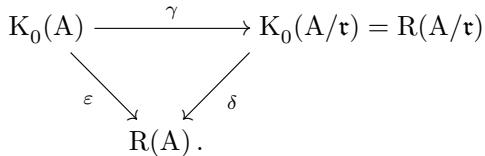
\includegraphics[keepaspectratio]{images/part002_05770a86.jpg}}

We denote the (finite) set of classes of simple A-modules by \(\mathcal{S}\) ; for every \(\lambda \in \mathcal{S}\) , choose a module \(S_{\lambda}\) of class \(\lambda\) and a projective cover \((P_{\lambda}, u_{\lambda})\) of \(S_{\lambda}\) (VIII, p.~175, Proposition 4). It follows from Proposition 6 of VIII, p.~176 that \(K_0(A)\) is a free \(\mathbf{Z}\) -module with basis the family \(([P_{\lambda}]_{\mathcal{P}(A)})_{\lambda \in \mathcal{S}}\) . Moreover, since \(S_{\lambda}\) is isomorphic to \(P_{\lambda} / \mathfrak{r}P_{\lambda}\) (VIII, p.~176), \(\gamma\) transforms the basis \(([P_{\lambda}]_{\mathcal{P}(A)})_{\lambda \in \mathcal{S}}\) of \(K_0(A)\) into the basis \(([S_{\lambda}])_{\lambda \in \mathcal{S}}\) of \(R(A / \mathfrak{r})\) . The isomorphism \(\delta\) transforms the basis \(([S_{\lambda}])_{\lambda \in \mathcal{S}}\) of \(R(A / \mathfrak{r})\) into the basis \(([S_{\lambda}])_{\lambda \in \mathcal{S}}\) of \(R(A)\) .

The Cartan matrix of A is the matrix \((a_{\lambda\mu})\) of the homomorphism of Z-modules \(\varepsilon: K_{0}(A) \to R(A)\) with respect to bases \(([P_{\lambda}]_{\mathcal{P}(A)})_{\lambda \in \mathcal{S}}\) of \(K_{0}(A)\) and \(([S_{\lambda}])_{\lambda \in \mathcal{S}}\) of \(R(A)\) . By definition, we have

\[
[ \mathrm{P} _ {\mu} ] = \sum_ {\lambda \in \mathcal {S}} a _ {\lambda \mu} [ \mathrm{S} _ {\lambda} ] \quad (\mu \in \mathcal {S})\tag{19}
\]

in the group R(A). In other words, \(a_{\lambda\mu}\) is the number of quotients isomorphic to \(S_{\lambda}\) in a Jordan--Hölder series of the A-module \(P_{\mu}\) .

Set \(\pi = \varepsilon \circ \gamma^{-1} \circ \delta^{-1}\) ; it is an endomorphism of the group R(A). If M is a finitely generated semisimple A-module and (P, \(u\) ) a projective cover of M, then we have \(\pi([M]) = [P]\) . By formula (19), the matrix of \(\pi\) with respect to the basis \(([S_{\lambda}])_{\lambda \in \mathcal{S}}\) of R(A) is simply the Cartan matrix of A.

